\chapter{引言}
\label{cha:intro}

\section{研究背景及意义}

随着科学技术的快速发展以及工业自动化程度的日益提升,越来越多的工业设备
朝着高度集成化、复杂化、智能化的方向发展;与此同时,这些设备所处的工作
环境的复杂程度也越来越高。其中有很大一部分是用在能源、电力、交通、冶金
等国民经济支柱型产业中。比如航天器制造和发射设备、尖端数控机床和工业机
器人、城市轨道交通设备等。我们在享受这些复杂系统给人们的生产生活带来的
便利的同时,也无法忽视其背后始终存在的重大问题——故障。

近几十年来,由于这一类复杂系统突发故障而直接引发的重大事故不胜枚举。
1998年6月,德国艾雪德高速列车由于长期金属疲劳形成的微细裂缝未得到及时
发现和处理,发生车轮爆裂,导致列车脱轨,死亡人数达100多人。2011年7月23
日,甬温线特大铁路交通事故的发生导致40人死亡,172人受伤,原因是列车的
自动保护系统发生故障。航空航天领域更是事故不断。1986年美国挑战者号航天
飞机刚起飞73秒即发生解体,造成7名机组人员丧命,原因是航天飞机起飞后,
右侧固体火箭助推器的O型环密封圈失效,使原本应该密封的固体火箭助推器内
的高热高压气体泄漏。2003年哥伦比亚号航天飞机由于外储箱上的绝热材料碎片
在发射过程脱落并击中左翼前缘,损坏了热防护系统,因此在执行任务期间发生
解体,机上所有7名宇航员瞬间遇难。此外,能源化工行业也频频传来噩耗。
1986年4月26日,乌克兰切尔诺贝利核电站4号反应堆发生爆炸,造成30人当场死
亡,8吨多强辐射物泄漏。此次核泄漏事故使电站周围6万多平方公里土地受到直
接污染,320多万人受到核辐射侵害,造成人类和平利用核能史上最大的一次灾
难。这些令人触目惊心的事故不断警示着我们,及早诊断出系统潜在的故障并及
时有效地进行处理,避免危险情况的发生,是保障工业系统安全稳定运行的关键
所在。目前,我们国家也非常重视这方面技术的研究和发展,在国家中长期规划、
国家自然科学基金委发展战略中都将故障诊断技术列为一个重要的发展方向。

\section{国内外研究现状}

系统在正常运行过程中,部分参数、状态或性能出现与期望不符的偏差时,我们
称系统发生了故障~\cite{van1997remarks}。通常情况下,在对系统健康状态的
监测过程中,故障诊断系统首先需要在被测对象发生故障时完成告警,其次需要
确定故障发生的类型和位置,最后需要估计出故障的严重程度。因此,一般将故
障诊断任务分解为以下三个方面:

1)故障检测(Fault Detection):确定系统是否发生故障,起到告警作用。

2)故障隔离(Fault Isolation):一旦故障检测阶段确认系统发生了故障,那
么需要进一步对故障的类型以及发生的位置进行确定。从而为维修过程提供辅助
信息,极大地提升系统设备的维修效率。

3)故障识别(Fault Identification):在完成故障隔离后,对故障的严重程度
进行估计,从而为采取何种维修手段提供重要的依据。

现有的故障诊断方法总体上可以分为两类:基于模型的故障诊断方法和基于数据
的故障诊断方法。

基于模型的故障诊断方法的基本思想是建立系统内部结构、行为或功能的数学模
型,并且基于此模型来预测系统的行为,然后将这些模型预测值与系统的观测值
进行比较~\cite{console1999model, davis1988model, mosterman1998comprehensive}。
如果预测值与观测值一致,说明系统正常;如果存在差异,那么利用这些差异去
搜索那些能够使模型预测值与系统观测值一致的各种可能行为的状态假设,这些状
态假设就是基于模型的故障诊断方法得出的诊断结果~\cite{wotawa2000debugging, friedrich1999model}。

在基于模型的故障诊断方法中,系统的模型是已知的,与之不同的是,数据驱动的
故障诊断方法仅仅取决于从系统中测量的数据。 由于计算机和信息技术的快速发
展,大量的测量数据可用于提取与系统当前状态相关的有用信息,并且对决策单元
做出更好的控制和优化方案提供支持~\cite{yin2012comparison}。因此,近些年来,
无论是在研究领域还是实际工业应用中,基于数据的故障诊断方法都受到越来越多
的重视。本文根据故障诊断模型在训练和预测过程中是否能够有效利用输入数据在
多个尺度上的特征,将基于数据的故障诊断方法划分为单一尺度的故障诊断方法和
多尺度的故障诊断方法。如图~\ref{fig:method_summary}所示。
\begin{figure}[ht]
  \centering
  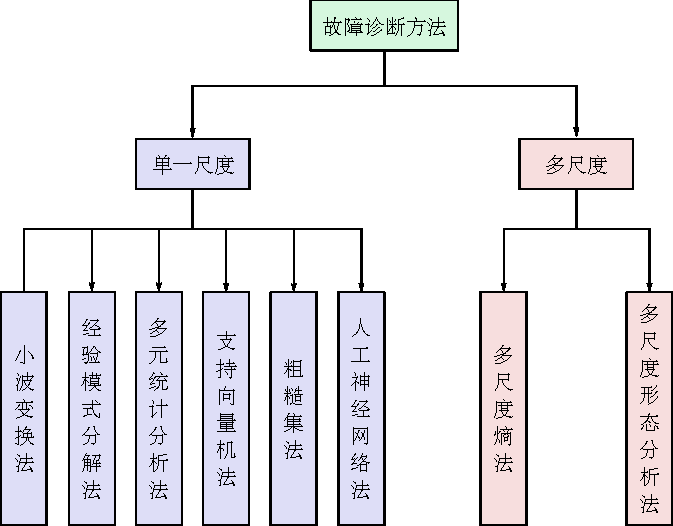
\includegraphics{method_summary}
  \caption{数据驱动的故障诊断方法分类}
  \label{fig:method_summary}
\end{figure}

\subsection{单一尺度的故障诊断方法}

目前大部分数据驱动的故障诊断方法都是基于单一尺度特征的。这一类方法有基于
信号处理的小波变换法(Wavelet Transform)、经验模式分解法(Empirical Mode
Decomposition, EMD)等;基于多元统计分析的方法如主元分析法(Principal
Component Analysis, PCA)、指定元分析法(Designated Component Analysis,
DCA)、独立元分析法(Independent Component Analysis, ICA)、核主元分析法
(Kernel Principal Component Analysis, KPCA)等;基于支持向量机(Support
Vector Machine, SVM)的方法;基于粗糙集(Rough Set,RS)的方法;基于人工
神经网络(Artificial Neural Network, ANN)的方法等。

1)小波变换法

小波变换是指使用有限长、快速衰减的、被称为母小波的振荡波形来表示信号的过
程,该波形被平移和缩放以匹配输入的信号。从提出到现在,小波变换在理论和应
用上都取得了巨大的发展,包括连续小波变换(Continuous Wavelet Transform,
CWT)、离散小波变换(Discrete Wavelet Transform)、小波包变换(Wavelet
Packet Transform, WPT)以及近些年提出的第二代小波变换(Second Generation
Wavelet Transform, SGWT)等,在各类系统的故障诊断中都得到了大量的应用。

文献~\inlinecite{zuo2005feature}将信号$x(t)$的CWT的小波系数作为初始特征,
结合PCA和ICA方法实现了齿轮箱的故障诊断。文献~\inlinecite{zhu2009synchronous}
将小波系数映射到极坐标系中,以增强由齿轮箱和轴承故障引起的周期性瞬变特征。
文献~\inlinecite{meltzer2004fault}同样使用极坐标系下的小波系数,提高了在
非平稳转速下运行的故障齿轮的检测能力。文献~\inlinecite{nagaraju2009application}
使用3维CWT提取信号在时频两域的特征,并结合相位角信息,提升了转子裂纹的检
测能力。文献~\inlinecite{rafiee2009use}将小波系数的自相关函数近似为简单的
正弦函数,并应用到齿轮箱故障诊断的特征提取过程中。文献~\inlinecite{peter2004machine}
基于遗传算法设计的精确小波分析过程进一步优化了小波系数,并应用于电动泵的
故障诊断中。

DWT的多分辨率分析能力使得它非常适合从采集自旋转机器上的非平稳信号中提取故
障相关的信息。文献\inlinecite{kim2007comparative}对转子系统的损伤检测进行
了比较研究,发现在包括短时傅立叶变换(Short Time Fourier Transform, STFT),
Wigner-Ville分布(Wigner-Ville Distribution, WVD)和DWT在内的各种时频技术
中,从加速和减速过程收集的振动信号中提取与裂纹状态有关的特征,DWT是其中最
有效的方法。文献~\inlinecite{omar2012dynamic}设计了一种动态的窗口小波多分
辨率分析方法,用于在嘈杂的环境中检测和定位齿轮缺陷。文献~\inlinecite{djebala2008detection}
在优化了小波多分辨率分析过程的基础上,使用峰度作为优化和评估标准,完成了
对轴承的故障检测。在许多研究中已经广泛采用基于DWT的去噪方法,来消除背景噪
声并增强测量信号中包含的故障相关信息。文献~\inlinecite{li2011virtual}设计
了一个基于DWT,自回归(Autoregressive, AR)模型和主成分分析(PCA)的齿轮
故障诊断方法,其中DWT的作用就是对原始振动信号进行去噪。

WPT具有更强的高频区信号分解能力,这使它成为检测和区分具有高频特性的瞬态分
量的最佳工具之一。在文献~\inlinecite{gao2006non}中,对比研究了WPT和其他时
频分析技术用于非平稳信号处理的效果,发现WPT能够识别轴承振动信号内由于缺陷
引发的瞬态分量,以及与缺陷增长的相变相关的频移。WPT也被用作预处理器将原始
信号分解成窄带信号,以提高希尔伯特 - 黄变换(Hilbert–Huang Transform)的
性能~\cite{peng2005comparison}。文献~\inlinecite{tian2010hybrid}使用WPT作
为预处理工具来减少WVD中通常存在的交叉干扰,增强了WVD在轴承故障诊断中的能
力。此外,从WPT的小波系数中提取的某些特征也被广泛用于直接表征机器的故障状
态。文献~\inlinecite{zarei2007bearing}将WPT应用于感应电动机定子电流信号,
并且提取子频带能量作为故障指标来检测轴承故障。文献~\inlinecite{li2008wavelet}
设计了一种基于小波的高阶统计方法用于滚动轴承的故障诊断,并且以WPT和DWT的
小波系数中提取的峰值作为损伤检测和分类的度量。

由于计算速度快,易于实施,近些年来将SGWT应用于旋转机械故障诊断的应用越来
越多。文献~\inlinecite{chen2007vibration}使用SGWT从水力电机的振动信号中提
取特征,对不同的活塞故障状态进行分类。文献~\inlinecite{he2009principle}通
过将SGWT应用于从数控机床的铣削过程测量的声发射信号来检测铣刀破损。文献~\inlinecite{bao2009anti}
为解决故障特征提取中的频率混叠问题,使用抗锯齿SGWT对信号进行了变换,
从而达到了较高的故障分类精度。文献~\inlinecite{hongkai2006gearbox}使用自
适应冗余SGWT分析了具有磨损故障的齿轮箱的振动信号,并从复杂背景中提取了脉
冲分量。同样,SGWT也经常被用来对信号进行去噪处理。在自适应SGWT的基础上,
文献~\inlinecite{li2012adaptive}设计了一种自适应形态梯度提升小波变换,以
增强由轴承缺陷引起的脉冲特征,同时抑制原始信号中包含的噪声。文献~\inlinecite{li2011mechanical}
提出了一种基于冗余非线性SGWT的去噪方法来去除机械故障信号中包含的噪声。

2)经验模式分解法

经验模式分解是黄锷(N. E. Huang)等人于1998年提出的一种自适应信号时频处理
方法~\cite{huang1998empirical}。EMD跟据数据自身的时间尺度特征进行信号分解,
并不需要预先指定基函数。这与分别建立在预先指定的谐波基函数和小波基函数上的
傅里叶变换与小波变换有本质的区别。这使得EMD在理论上可以应用于任何类型的信
号分解,因此尤其在处理非平稳和非线性的数据时,EMD具有非常明显的优势,得出
的结果具有很高的信噪比。EMD将复杂信号分解为有限个本征模函数(Intrinsic Mode
Function,IMF),各IMF分量包含了原始信号在不同时间尺度的局部特征信号。与STFT、
小波变换等方法相比,由于EMD的基函数是由数据本身分解得到,并且分解过程是基
于信号序列时间尺度的局部特性进行的,因此EMD是直观、后验和自适应的。

文献~\inlinecite{gaoqiang2007empirical}使用EMD分解将带有局部损伤的滚动轴
承所产生的高频调幅信号成分作为IMF分离出来,然后通过希尔伯特变换(Hilbert
Transform)得到其包络信号和包络谱,进而提取出滚动轴承故障的特征频率并完成
故障诊断。文献~\inlinecite{xu2009life}采用EMD分析轴承加速寿命试验的振动信
号,并研究了轴承寿命周期的演变趋势。文献~\inlinecite{junsheng2007application}
提出了基于EMD的能量算子解调方法,并用于轴承的故障诊断中。文献~\inlinecite{fan2008machine}
利用IMF的振幅加速能量来表示轴承和齿轮的故障特征。

EMD虽然有较好的处理非线性和非平稳信号的能力,但是同时也存在一定的问题,如
缺乏理论基础、端点效应、筛选停止标准、极值插值、模式混叠等。文献~\inlinecite{rato2008hht, chen2012signal, chen2012signal}
对此进行了详细的讨论。此外,也有一些针对此类问题的改进方法被提出。例如文献~\inlinecite{wu2009ensemble}
提出的集成经验模式分解(Ensemble Empirical Mode Decomposition, EEMD)方法,
通过在信号中增加噪声,解决了原始EMD方法模式混叠的问题。文献~\inlinecite{ai2009condition}
提出了一种基于EEMD和包络谱的方法,并可靠地诊断出了轴承的局部缺陷。文献~\inlinecite{zhouzhi2013eemd}
在使用EEMD对信号进行分解的基础上,使用互相关系数进行自适应重构从而突出故障
特征信号,并且使用谱峭度(Spectrum Kurtosis)确定带通滤波器的中心频率及带
宽,最后在滤波的结果上进行了能量算子解调谱分析,从而完成了滚动轴承的故障诊
断过程。文献~\inlinecite{dong2009sifting}提高了EMD筛选过程的效率,并实现了
轴承的内圈故障检测。

3)多元统计分析法

多元统计分析主要用于分析拥有多个变量的样本之间的关联性,或是厘清数据的
结构。基于多元统计分析的故障诊断方法的基本思想是:使用多元投影过程对多
变量样本空间进行分解,在子空间中构造反映空间变换的统计量,以计算出的统
计量为指标检测设备运行过程中的故障状态,基于多元统计分析的故障诊断方法
主要有PCA、 DCA、ICA、KPCA等。

PCA的提出最初是为了降低大型相关数据集的维数,同时仍然保留原始数据集中的
大部分信息~\cite{abdi2010principal}。由于其简单的形式和处理大量数据的能
力,PCA已经广泛应用于许多计算领域,如图像分析、特征提取、模式识别、数据
压缩和时间序列预测。此外,PCA在过程监控和故障诊断领域的应用也得到了极大
的发展。

运用PCA技术进行故障定位经典的方法是贡献图法~\cite{miller1998contribution},
当判断发生故障时,定义故障贡献度函数,分别计算多个变量的贡献度函数值,
并选取使函数最大的变量作为引起故障的变量。PCA技术用于故障分类的原理是
以包含各类故障信息的数据为训练数据,推导出指示数据变化最大的几个方向的
向量。将新观测的数据代入预先定义的故障分类判别式中,通常采用模式分类方
法中的后验判别式~\cite{duda2000pattern},依据达到最大的故障概率来对故障
进行归类。文献~\inlinecite{raich1996statistical}提出了以每类故障为训练
数据分别建立PCA模型,依次对新观测数据进行检验以确定属于哪种故障数据或新
的故障类。

由于PCA方法能检测出缓变的信号,文献~\inlinecite{gezhiqiang2007mewma}利
用PCA方法检测焚烧炉的早期故障,并设计出一个软件包,专门用于检测都市固体
废物焚烧炉(municipal solid waste incinerators, MSWIs)中的3种早期故障
–—局部烧穿、局部焦化和排渣故障,并已将其用于实际生产。为了解决过程变量
之间具有相关性的微小故障的诊断,文献~\inlinecite{gezhiqiang2007mewma}用
传统PCA结合单变量指数加权滑动平均(exponent weighted moving average,EWMA)
构成多变量EWMA–PCA(exponent weighted moving averageprincipal component analysis)
方法,详细分析了化工生成过程中各个统计量的统计性能指标及其影响因素,从
而检测出化工生产过程中的进料温度阶跃变化和冷却水阀的粘阻这两个微小故障。
与单纯的PCA方法相比,该方法对微小故障有较好的检测性能。考虑到过程中普遍
存在非高斯信息,文献~\inlinecite{gezhiqiang2008mcusum}把传统的单变量累计
和控制图(cumulative sum, CUSUM)扩展为多变量的形式,并与PCA和独立元分析
(independent component analysis,ICA)相结合,利用独立元分析–—主元分析
(independent component analysis-principal component analysis,ICA–PCA)
完整提取了生产过程中的非高斯和高斯信息,重构了统计量并建立了对应的统计限,
实现了微小故障的检测,并在TE平台上进行了验证。针对过程测量是动态的、多元
的且有限的情况,文~\inlinecite{majid2011aluminium}提出了多向主元分析法
(multiway principal component analysis,MPCA),实现了实时检测工业连续
铝电解过程中的早期故障–—阳极长包和阳极效应。为了实现系统中的多个耦合微小
故障的诊断,文献~\inlinecite{li2011virtual}首先利用小波变换实现对齿轮振
动信号的消噪,然后利用自回归模型(autoregressive, AR)提取故障特征集,最
后用PCA进一步将提取的特征集融合成一个特征以作为分类依据,实现对多个齿轮
故障的诊断。

由于传统的PCA是一种线性映射的方法,难于抽取过程变量的非线性特征,故基于
核主元分析法(kernel principal component analysis,KPCA)的故障诊断方法
应运而生。文献~\inlinecite{li2010gearbox}提出基于Gaussian核积分算子和PCA
的KPCA方法以诊断齿轮箱中的齿轮齿裂早期故障。文中首先通过Gaussian核积分算
子将齿轮箱的振动特征原输入空间非线性映射到高维空间,然后利用PCA进行早期
故障诊断。为了避免PCA的模式复合效应所带来的对多级微小故障辨识诊断失效的
问题,文献~\inlinecite{zhou2008dca}在基于DCA的投影框架下对多变量系统进行
多级微小故障的诊断。文中首先将观测数据矩阵关于多数显著变化模式进行DCA分
析,并剔除这些模式得到残差。然后针对不显著变化模式,对残差进行DCA分析,
并计算这些不显著故障模式的显著性以决定系统中是否发生微小故障。

多元统计分析的故障诊断方法基于系统运行过程中的测量数据,不需要对系统结构
深入了解,而且算法简单。目前该类诊断方法主要用于诊断工业过程中的缓变微小
故障。但由于该类方法诊断出来的故障难于解释以及实际系统的复杂性,还有很多
问题有待研究。

4)支持向量机法

基于数据知识的故障诊断方法不需要定量数学模型,而是利用人工智能技术,通过
算法训练使得计算机获得学习、推理以及决策等实现故障诊断的能力~\cite{venkatasubramanian2003reviewpart3}。
一般运用的知识包含系统结构知识、经验规则知识、工作状态知识、环境知识等。
基于数据知识的故障诊断方法可以定性方法和定量方法~\cite{venkatasubramanian2003reviewpart3, venkatasubramanian2003reviewpart1, venkatasubramanian2003reviewpart2}。
定性方法包括利用已知结果进行推理的图搜索方法和基于经验推断的专家系统方法,
其共同特点是诊断不一定完全基于定量化的数据,更多是基于状态、特征、属性等
非量化特征的变化。定量方法所需知识来源于大量的系统过程数据,典型的代表方
法有基于支持向量机的方法、基于粗糙集的方法以及基于人工神经网络的方法。

支持向量机(support vector machines,SVM)是20世纪90年代中期发展起来的机
器学习方法。SVM诊断故障的基本思想是:利用SVM的解决分类和函数回归问题的能
力,以及具有强大的处理少样本高维非线性问题的能力, 对故障特征进行分类,实
现故障被识别的目的~\cite{huqiao2006improved}。

为了提高单一的SVM的分类能力,文献~\inlinecite{lee2006diagnosis}提出了结
合ANN的SVM法以诊断变压器中的故障。该法运用克隆选择算法选择最优的输入特征
和径向基函数(radial basis function, RBF)内核函数,有效地提高了利用SVM
和ANN进行故障诊断的速度和精度。为了克服由于核参数和样本特征数选择不当而
产生的欠学习或过学习现象,文献~\inlinecite{huqiao2006improved}提出基于提
升小波包变换和集成支持向量机的故障智能诊断方法。该方法首先用提升小波包变
换提取信号敏感频带特征,进而通过对敏感带中的小波包系数进行包络解调分析检
测出故障特征频率,然后通过距离评估技术选取最优特征集,最后将最优特征输入
到SVM进行故障诊断。该方法提高了故障诊断的准确率,并将其用于滚动轴承内外
圈故障的诊断。针对机械故障诊断中缺乏大量故障样本进行训练的问题,文献~\inlinecite{liweihua2010graph}
提出了基于图论和直推式SVM相结合的方法以诊断齿轮齿面轻微剥落的故障。该方
法首先对振动信号进行分析并提取时域特征指标,然后用主元分析对提取的特征进
行选择,用图论方法对选择后的特征数据进行处理,最后用梯度下降法训练直推式
SVM,实现故障检测和分类。

SVM是解决高维非线性问题强有力的工具,且SVM更适用于少样本情况下的故障诊断
和检测。但SVM参数以及样本的完备性和代表性对故障分类的性能有很大的影响,
且单一的SVM容易产生由于核参数和样本特征数选择不当而引起的欠学习或过学习
现象,故SVM在进行故障诊断时通常和其他的方法相结合来提高诊断的准确率。

5)粗糙集法

由于传统的Pawlak粗糙集(RS)是基于非空有限集的,其对象的属性值是离散的。
而在大多数问题中,对象的属性值在确定论域内是连续的,且其中的一些属性值
是模糊的。于是模糊RS被用于故障的诊断。文献~\inlinecite{hao2006improved}
用模糊RS的方法诊断变压器中的早期故障,所提出的方法不仅能处理不完全信息
输入和规则简约,而且能对其连续属性阈值进行模糊化,从而有效地诊断出变压
器早期故障的类型及故障程度。考虑到重叠故障模式可能表示一类早期故障或者
是一类多故障的样本子集,文献~\inlinecite{zhang2012vibrant}提出一种新的
改进的RS与一对一多类SVM方法。通过利用RS描述分类问题中的重叠区域以及利用
SVM的泛化能力,诊断出水轮发电机组的早期故障.

基于RS的故障诊断方法能发现数据间的潜在规律,并且能够处理不完备的数据信
息以及对象的属性值在确定论域内是连续的情况,具有较强的数据分析能力。

6)人工神经网络法

用神经网络(artificial neural network,ANN)进行微小故障诊断的基本思想
是:根据大量历史样本数据建立故障识别和分类的映射,通过网络训练得到网络
权值,并将此用于发现观测数据样本异常行为,实现对故障的诊断与隔离。

文献~\inlinecite{chow1988incipient}最早提出用ANN法诊断直流电机中的故障。
经过几十年的发展,各种ANN方法被应用于微小故障的诊断领域。文献~\inlinecite{watanabe1989incipient}
提出用两阶段多层ANN诊断化工过程中由于组件性能退化产生的故障,其中:第1
阶段用于辨识当系统的反馈信号含有测量噪声情况下的故障原因;一旦故障被识
别出,第2阶段将估计故障的程度。文献~\inlinecite{chow1991methodology}提
出一种用ANN在线检测单相鼠笼式异步电动机中故障的方法,其在线的故障检测分
为两部分:第一部分使用噪声/干扰滤波神经网络(disturbance and noise filter artificial neural network,DNF-ANN)
滤除测量瞬态值的同时保持测量稳态值;第二部分基于从电机中采集来的数据,
利用高阶ANN在线检测单相鼠笼式异步电动机的匝间定子绝缘故障和轴承磨损这两
种常见早期故障。考虑到ANN不能提供关于电机或者故障检测过程中的启发式知识,
文献~\inlinecite{goode1994hybrid}提出使用混合模糊/ANN方法检测单相感应电
机早期轴承故障。该方法利用ANN的学习能力检测电机是否发生故障, 通过使用模
糊规则和模糊隶属函数获得对启发式知识更好的理解。为了提高微小故障诊断的
快速性和准确性,文献~\inlinecite{wang2003extension}将可拓理论和ANN相结合,
提出了用可拓神经网络方法(extension neural network, ENN)诊断故障。 该方
法减少了训练时间、提高了映射能力和容错能力,快速而准确地诊断出变压器中几
种常见的故障。当训练样本和输入信息维数过大时,ANN通常不能简化输入信息维数,
这将会导致ANN的结构复杂、训练时间长。针对这一问题, 文献~\inlinecite{dong2008rough}
提出将粗糙集和模糊小波神经网络(fuzzy wavelet neural network, FWNN)、最
小二乘(least square, LS)加权融合算法相结合的诊断方法。该方法利用粗糙集
的知识简约能力简化小波神经网络输入,利用FWNN良好的分类诊断能力并结合LS加
权融合算法诊断出电力变压器中的热故障和放电故障。考虑到采集的信号受到噪声
污染以及不同运行时段信号可能有不同的稳态值, 文献~\inlinecite{rakic2010early}
针对磨煤机的故障提出基于自组织映射ANN的故障检测方法。该方法首先对磨煤机
的动量和转速等实时数据进行预处理,训练和使用自组织映射ANN检测火电厂磨煤
机中由于输入仓煤堵塞所导致的输出燃料混合物下降的故障。

由于ANN具有强的非线性拟合能力、自学习能力、自组织能力和容错能力,故在故障
诊断中得到了广泛的应用。但用ANN建模需要大量的样本数据, 样本的完备性和准确
性对建模有直接的影响,从而影响故障诊断的效果。另外,传统的ANN建模对偏差很
敏感, 任何微小的偏差或扰动都会导致拟合精度的下降甚至使之完全丧失拟合能力~\cite{zhangzhengdao2004ann},
这些都会影响到故障的诊断效果。此外,ANN对学习和诊断结果的可解释性相对较差。
因此, 出现了将ANN与其他方法融合的故障诊断方法。

\subsection{多尺度的故障诊断方法}

\subsubsection{多尺度熵算法}

时间序列的复杂度可以通过多种方法进行研究,例如近似熵~\cite{valenza2014inhomogeneous}
和样本熵~\cite{yentes2013appropriate}。然而,这些方法并没有考虑存在于实际
物理系统中的多种时间尺度。因此,Costa等人于2002年提出了多尺度熵(MSE)方法
,通过计算不同尺度下序列的样本熵,来表示时间序列在不同尺度下的复杂性~\cite{costa2002multiscale}。

由于MSE的计算依赖于样本熵,因此在介绍MSE的计算方法之前,我们先来介绍样本熵。
对于一个长度为$N$的原始时间序列$x=\{x_1, x_2, ..., x_N\}$,记$x(i)=\{x_i, x_{i+1}, ..., x_{i+m-1}\}$
为原始序列$x$的第$i$个长度为$m$的子序列。样本熵定义为一个条件概率,它量化长
度为$m$的子序列与另一个相同长度的子序列相等(在r的误差容忍范围内)时,将它
们的长度增加为$m+1$后仍然相等的概率。我们将$m$称为嵌入维数。两个子序列之间
距离定义为对应元素差值绝对值的最大值。例如,序列$x(i)$与序列$x(j)$之间的距
离$d_{ij}$定义为~\ref{equ:chap1:l1_norm}式。
\begin{equation}
  \label{equ:chap1:l1_norm}
  \begin{aligned}
    d_{ij} = & d(x(i), x(j)) \\
    = & \max_{k=0}^{m-1}|x(i+k)-x(j+k)|
  \end{aligned}
\end{equation}

将两个长度为$m$的子序列相等(在r的误差容忍范围内)的概率记作$B^m(r)$。那么
$B^m(r)$可以如下计算:对每个$i$,计算$x(i)$与其余子序列$x(j)(j=1,2,...,N-m; j\neq i)$
的距离$d_{ij}$,并统计$d_{ij}$小于$r$的平均个数,如~\ref{equ:chap1:bmr}式所
示。
\begin{equation}
  \label{equ:chap1:bmr}
  B^m(r)=\frac{1}{(N-m)(N-m-1)}\sum_{i\neq j}\theta(r-d_{ij})
\end{equation}

其中$\theta(x)$是单位阶跃函数:
\begin{equation}
  \label{equ:chap1:step_func}
  \theta(x) = \left\{
  \begin{aligned}
    1 &, x > 0 \\
    0 &, x \leq 0
  \end{aligned}
  \right.
\end{equation}

从而样本熵的定义可以表示为~\ref{equ:chap1:sample_entropy}式。
\begin{equation}
  \label{equ:chap1:sample_entropy}
  \text{SampEn}(m, r) = \lim_{N\to\infty}-\ln\frac{B^{m+1}(r)}{B^m(r)}
\end{equation}

在$N$为有限值时,~\ref{equ:chap1:sample_entropy}式可以写成~\ref{equ:chap1:sample_entropy_finite}
式。
\begin{equation}
  \label{equ:chap1:sample_entropy_finite}
  \text{SampEn}(m, r, N) = -\ln\frac{B^{m+1}(r)}{B^m(r)}
\end{equation}

根据Trunkvalterova等人~\cite{trunkvalterova2008reduced}的研究,嵌入维度$m$
通常取2,误差容忍度$r$通常取原始时间序列标准差的0.15倍。正常和周期信号的理
论样本熵为0,而不相关的随机信号具有最大样本熵(该值取决于信号长度)。

MSE算法由以下两个步骤组成~\cite{costa2002multiscale, costa2005multiscale}:

1)通过一系列粗粒度(coarse grained)过程,计算原始时间序列在不同尺度上的
一组表示序列。在尺度为$\tau$的粗粒度过程中,将给定时间序列的每个长度为$\tau$
的连续不重叠区间内的数据点进行平均,所得的结果作为尺度$\tau$下的表示序列。
例如,对于一个长度为$N$的离散信号$\{x_1,...,x_i,...,x_N\}$,原始时间序列的
粗粒度表示序列$\{y^{(\tau)}\}$计算方式如~\ref{equ:chap1:coarse_grained}式
所示。
\begin{equation}
  \label{equ:chap1:coarse_grained}
  y^{(\tau)} = \frac{1}{\tau}\sum_{i=(j-1)\tau + 1}^{j\tau}x_i , 1\leq j\leq N/\tau
\end{equation}

尺度为$\tau=1$时,粗粒度表示序列$y^{(1)}$对应原始信号。序列$y^{(\tau)}$的
长度为$N/\tau$。

2)计算每个粗粒度表示序列$y^{(\tau)}$的样本熵,得到由r个样本熵值构成的序
列,即为MSE的结果。对每个粗粒度表示序列求样本熵时,使用相同的误差容忍度$r$。

从提出以来,MSE已经成为量化信号复杂度的普遍方法。由于MSE对非线性、非平稳
序列有良好的处理能力,而且具有多尺度特征的提取能力,因此已经成功应用于很
多研究领域。在故障诊断领域也得到了非常广泛的应用。

文献~\inlinecite{zhang2010bearing}计算了20个尺度上的MSE,并在此基础上构造
了最大值、最小值、算术平均值、几何平均值以及标准差这5个统计值作为特征,结
合自适应模糊神经推断系统(Adaptive Neuro-fuzzy Inference System, ANFIS)
实现了对滚动轴承的故障诊断。文献~\inlinecite{zhengjinde2012mse}使用MSE算法
对滚动轴承的振动信号进行特征提取,并比较了MSE算法相对于单一尺度下的样本熵
算法的优势,最后使用支持向量机作为分类器,完成了滚动轴承故障类型的识别。文
献~\inlinecite{liu2014fault}使用局部平均分解(Local Mean Decomposition, LMD)
将滚动轴承的非平稳振动信号分解成多个项的乘积,并计算各乘积项的MSE作为特征,
实现了多种类型的故障状态的识别。文献~\inlinecite{zhanglong2014mse}基于时间
序列的MSE的偏度(Skewness)和均值构造了一个故障程度定量描述指标——多尺度熵
偏均值(Partial Mean of Multiscale Entropy, PMME),实现了轴承故障程度的评
估,并且能够跟踪故障发展的趋势。

在MSE的基础上,也有很多研究人员针对其存在的一些问题提出了相应的改进算法。
文献~\inlinecite{humeau2015multiscale}对原始的MSE算法以及很多不同的改进算
法进行了综述。例如文献~\inlinecite{xie2008measuring}提出,MSE算法所依赖的
样本熵的计算过程中用到了阶跃函数,从而引入了不连续因素,因此使用连续的Sigmoid
函数来替代阶跃函数,提出了多尺度模糊熵(Multiscale Fuzzy Entropy, MFE)算
法。

文献~\inlinecite{zhengjinde2014mfe}使用多尺度模糊熵对滚动轴承的振动信号
进行特征提取,并使用SVM作为分类器,实现了滚动轴承外圈、内圈和钢球3种故障
状态的识别。文献~\inlinecite{zhengjinde2016cmfe}针对MSE粗粒化方式的不足,
提出了复合多尺度模糊熵(Composite Multiscale Fuzzy Entropy, CMFE)算法来
度量时间序列的自相似性和复杂性。CMFE综合了序列在同一尺度下多种粗粒化方式
的结果,获得更加稳定和一致的特征。在此基础上,结合Fisher得分进行特征选择
并通过SVM进行分类,完成了对滚动轴承的故障诊断过程。

\subsubsection{多尺度形态分析}

数学形态学(Mathematical Morphology, MM)~\cite{haralick1987image}是一种
非线性分析方法,最初是为图像处理而设计的,后来在信号分析等领域也得到了广
泛的应用。通过对原始信号进行形态分解~\cite{pitas1990morphological},复杂
信号可以从背景中分离出来,并分解为保留了原始信号形态特征的多种分量。信号
形态处理的基本思路是通过一些形态变换来改变信号的形状。基本的形态变换算子
有扩张、腐蚀、开、闭运算。

令$f(n), n={0, 1, ..., N-1}$表示一个一维信号,$g(n), n={0, 1, ..., M-1}$
表示一个结构元素(Structuring Element, SE),腐蚀和扩张算子可以定义为~\ref{equ:chap1:erosion_dilation}
式。
\begin{equation}
  \label{equ:chap1:erosion_dilation}
  \begin{aligned}
    (f\ominus g)(n) = & \min_{m=0}^{M-1}\left[f(n+m)-g(m)\right] \\
    (f\oplus g)(n) = & \max_{m=0}^{M-1}\left[f(n-m)+g(m)\right]
  \end{aligned}
\end{equation}

其中$\ominus$表示腐蚀运算,$\oplus$表示扩张运算。基于这两种运算,两外两
种形态变换算子开、闭运算可以由~\ref{equ:chap1:opening_closing}式定义。
\begin{equation}
  \label{equ:chap1:opening_closing}
  \begin{aligned}
    (f\circ g)(n) = & (f\ominus g\oplus g)(n) \\
    (f\bullet g)(n) = & (f\oplus g\ominus g)(n)
  \end{aligned}
\end{equation}

其中$\circ$表示开运算,$\bullet$表示闭运算。表~\ref{tab:morphological_operator_effect}
列出了四种基本形态运算对信号脉冲的影响。
\begin{table}[htb]
  \centering
  \begin{minipage}[t]{0.6\linewidth}
  \caption{四种基本形态运算对信号脉冲的影响}
  \label{tab:morphological_operator_effect}
    \begin{tabularx}{\linewidth}{XXX}
      \toprule[1.5pt]
      形态运算 & 正脉冲 & 负脉冲 \\\midrule[1pt]
      腐蚀 & 抑制 & 平滑 \\
      扩张 & 平滑 & 抑制 \\
      开运算 & 抑制 & 保留 \\
      开运算 & 保留 & 抑制 \\
      \bottomrule[1.5pt]
    \end{tabularx}
  \end{minipage}
\end{table}

此外,还有其他一些由这些运算组合而成的形态运算,例如比较常用的平均算子AVG
和梯度算子DIF,如式~\ref{equ:chap1:average_difference}所示。
\begin{equation}
  \label{equ:chap1:average_difference}
  \begin{aligned}
    AVG(f) = & (f\bullet g + f\circ g)/2 \\
    DIF(f) = & f\bullet g - f\circ g 
  \end{aligned}
\end{equation}

在实际应用中,通常根据信号处理的不同场景选择或组合使用合适的形态运算。
SE是形态分析的另一个关键部分。通常,只有当所关心的信号成分的尺度和形
状与SE的尺度和形状匹配时,才能在经过形态运算后保留下来。因此,应该根
据待分析的信号来选择SE的形状、长度和高度(振幅)。SE的形状可以从规则
到不规则的曲线变化,例如水平线、三角和半圆等,如图~\ref{fig:se_shape}
所示。
\begin{figure}[ht]
  \centering
  \subcaptionbox{呈水平状的SE\label{fig:se_shape_flat}}
  {
\includegraphics[width=3cm]{se_flat}}
  \hspace{4em}
  \subcaptionbox{呈三角状的SE\label{fig:se_shape_triangular}}
  {
\includegraphics[width=3cm]{se_triangular}}
  \hspace{4em}
  \subcaptionbox{呈半圆状的SE\label{fig:se_shape_semicircular}}
  {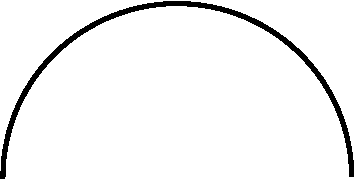
\includegraphics[width=3cm]{se_semicircular}}
  \caption{不同形状的SE}
  \label{fig:se_shape}
\end{figure}

SE的尺度,包括长度和高度对于一维信号的形态分析也很重要。传统的形态分
析是在单一尺度下进行的,其中SE是根据先验知识来设定的。然而这些先验知
识并不是在任何情况下都适用,而且很多问题中我们很难获取到这些先验知识。
因此,为了从信号中提取不同尺度的形态特征,需要进行多尺度形态分析。多
尺度形态分析是使用多种尺度的一组SE,分别对原始信号进行形态分析,从而
获得多种尺度下特征的过程。

文献~\inlinecite{haorujiang2008mmf}使用形态开运算对滚动轴承振动信号
进行多尺度形态分解,并计算不同尺度下的形态谱,然后在此基础上计算不同
尺度下信号的形态谱熵值,进而以此为特征完成了不同故障类型的定量区分。
文献~\inlinecite{wangbing2013mmf}使用多尺度形态分析将电机滚动轴承的
振动信号分解到多个尺度上,并在此基础上计算能谱熵和奇异谱熵作为特征,
结合灰色关联分析,完成了对电机轴承退化状态的评估。文献~\inlinecite{libing2011adaptive, li2011weighted}
使用梯度形态算子和水平状SE对滚动轴承的振动信号进行了多尺度形态分解,
并且定义了一种自适应的权值计算方法,对分解得到的各尺度下的信号进行
加权,使得小尺度下分解得到的信号具有较小的权重,大尺度下分解得到的
信号具有较大的权重,从而在保留原始信号细节的同时有效地抑制了噪声。
从实验结果可以看出这种方法能够有效地从故障轴承的振动信号中提取出特
征冲击信号。文献~\inlinecite{tangguiji2015adaptive}使用Top-Hat形态
算子对滚动轴承的振动信号进行多尺度形态分析,并在此基础上通过计算特
征幅值能量比(Feature Amplitude Energy Radio, FAER)来自适应地选择
最佳尺度,成功地应用于轴承的故障增强检测当中。
